\documentclass{deliverablereport}

\usepackage[style=alphabetic,backend=bibtex]{biblatex}
\addbibresource{report.bib}
\addbibresource{../../lib/publications.bib}

\usepackage{xparse}
\usepackage{etoolbox}
\usepackage{caption}
\graphicspath{{events/}}
 \ExplSyntaxOn

\newcounter{eventcounter}

\newenvironment{event}[7]{
\vspace{0.5cm}
\refstepcounter{eventcounter}
\label{event-#2}
\addcontentsline{toc}{subsection}{\hspace{3ex}-\ Event~\theeventcounter -~ #1}


\noindent\textbf{Event~\theeventcounter -~ #1}\newline % title

\noindent #3 \newline % location and date

\noindent ODK~partners~involved:~ \clist_map_inline:nn{#4}{\site{##1}~}\newline %partners

\ifx&#5&%
      % no participant #
\else
\noindent #5~participants~
\ifx&#6 &%
    % no odk participant
\else 
~(including~#6~from~within~ODK)\newline
\fi
\fi

\ifx&#7&%
      % no website
\else
\noindent \url{#7}\newline
\fi



}{\begin{center}\noindent\rule{4cm}{0.4pt}\end{center}}

 \ExplSyntaxOff


\deliverable{dissem}{workshops-4}
\duedate{31/08/2019 (M48)}
\deliverydate{31/08/2019}
\author{Viviane Pons et al.}

\begin{document}
\maketitle
\githubissuedescription
\newpage
\tableofcontents
\newpage

\section{Development workshops}

\TODO{EDIT}
We call a development workshop an event with a restricted number of participants
who meet to work on a specific task. These workshops are an inherent part
of \ODK development process as described in \taskref{dissem}{devel-workshops}:
 they bring together
developers from within and outside of \ODK and allow effective work
and discussions on many technical aspects. They also participate in building
and maintaining a community of developers inside \ODK and within the
open-source communities we belong to.

Throughout years 2 and 3 of the project, we have had 15 workshops dedicated mostly
to development. Some of them also included a training approach. 



\section{Dissemination and outreaching activities}

\TODO{EDIT}

We describe here all activities related to \taskref{dissem}{dissemination}:
these are all events oriented towards dissemination, training, and outreach. This
includes events organized or co-organized by \ODK and also
participating in external events and many communication activities.

\subsection{Training workshops and events}

\begin{event}{SageMath classes in Crete}{crete}{Heraklion, March. 4-6, 2019}{PS}{10}{1}{}

\textbf{Main goals.} We organized a series of SageMath classes in the mathematical department of the Univeristy of Crete.

\textbf{ODK implication.} OpenDreamKit funded the trip of Viviane Pons to give the classes.

\textbf{Event summary.} A series of three classes was organized throughout the week. This was open both to students (from undergrad to PhD) and researchers of the math department of the Univeristy of Crete. The classes consisted of SageMath tutorials to allow the attendees to discover the software at their own pace. We used Jupyter notebooks with a focus on math related problems.

\textbf{Results and impact.} The students enjoyed the tutorials a lot. It was actually used as a starting point for more regular sessions tutored by their local teacher Eleni Tzanaki. We are now confident that SageMath will be taught at Univeristy of Crete as part of the math program.  The meeting was also an occasion to prepare the up-coming Women in Sage event also organized in Crete. 

\end{event}



\subsection{Organization of Sage Days in established mathematical communities}

One goal of \ODK is to support local communities of researchers
and developers who contribute to the open-source software related to
the project. For \Sage, this means supporting the organization of Sage-Days
workshops that arise from within all the different mathematical communities. The main 
goal of these workshops is mostly to improve the Sage coverage of some mathematical
area. They also play a major role in training and communication. The
impact for \ODK can be summarized this way:

\begin{itemize}
\item \textbf{Making \ODK known to the end users}: by supporting Sage Days,
\ODK makes itself known to the Sage community and can
thus share the many developments of the project.

\item \textbf{Improving the overall quality of Sage}: by fostering researchers
in specific areas, Sage Days help bring interesting mathematics into
the software, which is beneficial for Sage and so \ODK.

\item \textbf{Training, bringing more user}: Sage Days are the perfect place
for new comers, especially students, to get their first experience with the software.

\item \textbf{Fostering a community}: Sage Days are helping making Sage a vibrant
community, which is vital for the success of \ODK.
\end{itemize}



\subsection{Training activities in developing countries}


\subsection{Women in \ODK}

\TODO{EDIT}
\ODK is aware of the gender gap that exists in science in general
and more specifically in software development. We have been organizing
events to support specifically women developers, engineers and scientists.

\begin{event}{Sage Days 98 : Women in Sage}{SD98}{Archanes (Greece), April 8 -- April 12, 2019}{PS}{22}{1}{https://opendreamkit.org/2019/06/28/WomenInSage/}

\textbf{Main goals.} The main goal of the event was to initiate more women to the software \Sage to reduce the gender gap in mathematics software
development. Each participant had to propose a mathematic development project to be carried out during the week.

\textbf{\ODK implication.} The event was initiated by Viviane Pons from \ODK and co-organized with Eleni Tzanaki (University of Crete). It was funded solely by \ODK which covered: lodging for the participants (rented houses), food, and transportation for many of the participants.

\textbf{Event summary.} The event was organized as a workshop where every participant could work on their own project to develop their coding skills. We started the week with an introduction to Sage and some tutorials. Then each participant gave a 5 minute talk about their own research. After that, we worked on different projects, organizing status reports every day. In particular, we ran a group specifically to produce new contributions to Sage.

\textbf{Demographics.} All participants were women coming from 8 different countries (France, Belgium, Germany, Greece, UK, US, Romania and Peru), as per institutions, and more if we count nationalities (Australia, Lebanon, Spain). About half of them could be considered Sage beginners. We had 1 master student, 14 PhD students, 2 postdocs, and 5 \textit{Maîtresses de conférences} or assistant professor or lecturer.

We were supposed to also welcome 3 women from Nigeria but they were sadly not able to obtain their visas on time.

\textbf{Results and impact.} A full report on the impact of this
workshop can be read on our website:
\centerline{\url{https://opendreamkit.org/2019/06/28/WomenInSage/}}
The main goal was to make the participants more confident into their programming skills and more prone to become Sage contributors and attend classical Sage Days. It was a big success in that regard. Indeed, before the conference, only 17\% of the participants had attended Sage Days more than once and 50\% had never heard of it. After, the conference, 94\% rated 3 or more out of 5 the chances that they would attend Sage Days event in the future. 100\% of the participant rated 3 or more out of 5 the impact of the workshop on their future career and 100\% said they met interesting people. Additionally, work was done on 5 Sage issues from of which 3 have been merged into Sage source code already.

\begin{figure}[ht]
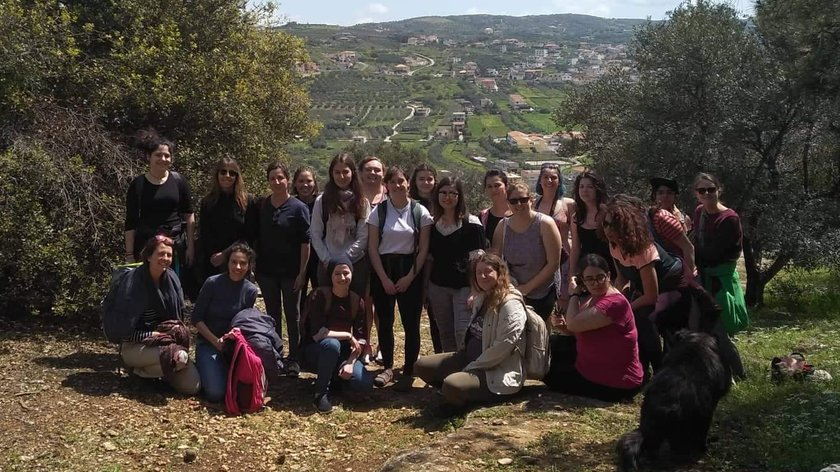
\includegraphics[scale=.3]{group_photo_head.jpeg}
\caption*{Women in Sage in Archanes}
\end{figure}



\end{event}


\subsection{Organization of research workshopts}


\subsection{Communication and participation to external events}

\begin{event}{Keynote at PyconFr}{pyconfr}{Lille (France), Oct. 6, 2018}{PS}{400}{1}{https://www.pycon.fr/2018/}

\textbf{Main goals.} PyConFr is the annual gathering of the French python community. 

\textbf{ODK implication.} Viviane Pons was invited to be the opening keynote of the conference.

\textbf{Event summary.} She gave a 30 minutes talk on ``Science and Open-Source: what do we learn from each other'' This was an occasion to discuss the many interactions between research and open-source development and highlight the role of projects such as OpenDreamKit.

\textbf{Results and impact.} The talk was well received by the python community with many positive feedbacks.

\end{event}



%\newpage\printbibliography

\end{document}

%%% Local Variables:
%%% mode: latex
%%% TeX-master: t
%%% End:
